\subsection{Funkcinis-reaktyvus programavimas}

Daugiausia remtąsi \cite{Survey}.

\subsubsection{Įvadas}

Funkcinis-reaktyvus programavimas, toliau vadinamas tiesiog FRP, yra būdas modeliuoti reaktyvų - besikeičiančius laiko tekmėje bei reaguojančius į išorinį stimulą - elgesį visiškai funkcinėse programavimo kalbose. FRP leidžia deklaratyviu ir paprastu būdu modeliuoti sistemas, kurios turi reaguoti į duomenis bėgant laikui.

\subsubsection{Pagrindinis tiklas}

Pagrindinis funkcinio-reaktyvaus programavimo tikslas:

\begin{itemize}

	\item saugus programavimas - kompiliatorius turi kiek įmanoma patikrinti programų korektiškumą;

	\item efektyvus programavimas - programos turėtų veikti realiu laiku, todėl efektyvios ir optimizuotos operacijos yra būtinos;

	\item komponavimas - FRP leidžia kurti programas iš smulkesnių programų, o ne orientuotą į problemą, vientisą kodą.

\end{itemize}

\subsubsection{Sąvokos}

Pagrindinės FRP sąvokos yra:

\begin{itemize}

	\item signalai arba elgsena - besikeičiančios laike reikšmės;

	\item įvykiai - kolekcija momentinių reikšmių arba laiko-reikšmės poros.

\end{itemize}

FRP pasiekia reaktyvumą naudodamas konstrukcijas, kurios tiksliai apibrėžia kaip signalai arba elgsena pasikeičia reaguodami į įvykius. Tai yra pagrindinis būdas išreiškiant bei realizuojant elgseną. Kitu būdu, elgsena gali būti laiko semantinės funkcijos\footnote{http://msdl.cs.mcgill.ca/people/tfeng/docs/as/node5.html}, kuriose laikas yra pakeičiamas kilus įvykiui.

\subsubsection{Semantika}

\subsection{Įvykių kaupimas}

Šiame skyriuje yra aprašomos žinios apie įvykių kaupimą, pliusus ir minusus, įvykių srautus bei įvykių kaupimą funkciniame programavime remiantis Vaughn Vernon surinkta ir aprašyta informacija \cite{vernon2013implementing}.

\subsubsection{Įvadas}

Kartais verslui svarbu fiksuoti objekto pasikeitimus domeno modelyje\footnote{http://en.wikipedia.org/wiki/Domain\_model}. Šiuos pasikeitimus galima stebėti skirtingais būdais. Įprastai yra pasirenkama stebėti kai esybė\footnote{http://en.wikipedia.org/wiki/Entity} yra:

\begin{itemize}

	\item sukurta,

	\item paskutinį kartą modifikuota

	\item bei kas atliko modifikaciją.

\end{itemize}

Tačiau šis būdas nepateikia jokios informacijos apie vienkartinius pasikeitimus.

Atsiradus poreikiu stebėti pasikeitimus detaliau, verslas reikalauja dar daugiau metaduomenenų\footnote{http://en.wikipedia.org/wiki/Metadata}, ko pasekoje tokie faktai kaip individualios operacijos laiko tekmėje bei jų įvykdymo laikas tampa svarbūs. Šie poreikiai verčia įvesti audito žurnalą fiksuoti labai tikslias panaudojimo atvejų metrikas, tačiau pastarasis būdas turi apribojimų. Jis gali atskleisti dalį informacijos apie tai kas nutiko sistemoje, leisti rasti bei ištaisyti dalį riktų bei klaidų programinėje įrangoje, bet audito žurnalas neleidžia patikrinti domeno objekto būsenos prieš ir po tam tikrų pasikeitimų. O jeigu būtų galima išgauti daugiau informacijos iš pasikeitimų stebėjimo?

Visi programinės įrangos kūrėjai susiduria su labai tiksliu pasikeitimų stebėjimu. Įprastas ir populiarus pavyzdys yra išeities kodo saugyklos, tokios kaip CVS\footnote{http://www.nongnu.org/cvs/}, Subversion\footnote{http://subversion.apache.org/}, Git\footnote{http://git-scm.com/} arba Mercurial\footnote{http://mercurial.selenic.com/}. Visos šios pataisų valdymo sistemos leidžia stebėti pirminių failų pasikeitimus. Įrankiai leidžia peržiūrėti išeities kodo artefaktus nuo pačios pirmosios pataisos iki paskutinės. Kai visi išeities failai yra nusiunčiami į pataisų kontrolės sistemą, ši gali stebėti pasikeitimus viso programinės įrangos kūrimo gyvavimo ciklo metu.

Jeigu šis principas būtų pritaikytas vienai esybei, tada vienam agregatui\footnote{http://martinfowler.com/bliki/DDD\_Aggregate.html} bei galiausiai kiekvienam modelio agregatui, galima suprasti kokią naudą atneša sistemos objektų pasikeitimų stebėjimas:

\begin{itemize}

	\item Kas būtent nutiko modelyje, jog agregato egzempliorius buvo sukurtas?

	\item Kas nutiko agregato egzemplioriui bėgant laikui? (Operacijų požiūriu)

\end{itemize}

Turint visų atliktų operacijų istoriją, galima palaikyti laikinus modelius. Toks kaitos stebėjimas yra įvykių kaupimo principas. \ref{pic:es} diagramoje pateika šio principo aukšto lygio reprezentacija. Agregatai publikuoja įvykius, kurie yra išsaugomi įvykių saugykloje ir naudojami sekti modelio būsenos pasikeitimus. Verta paminėti, jog įvykiai reprezentuoja tam tikrą būsenos pasikeitimą bėgant laikui, todėl jie nėra atnaujinami arba ištrinami. Saugykla nuskaito įvykius iš įvykių saugyklos ir pritaiko juos vieną po kito taip atkurdama agregato būseną. 

\begin{figure}[ht]
	\centering
	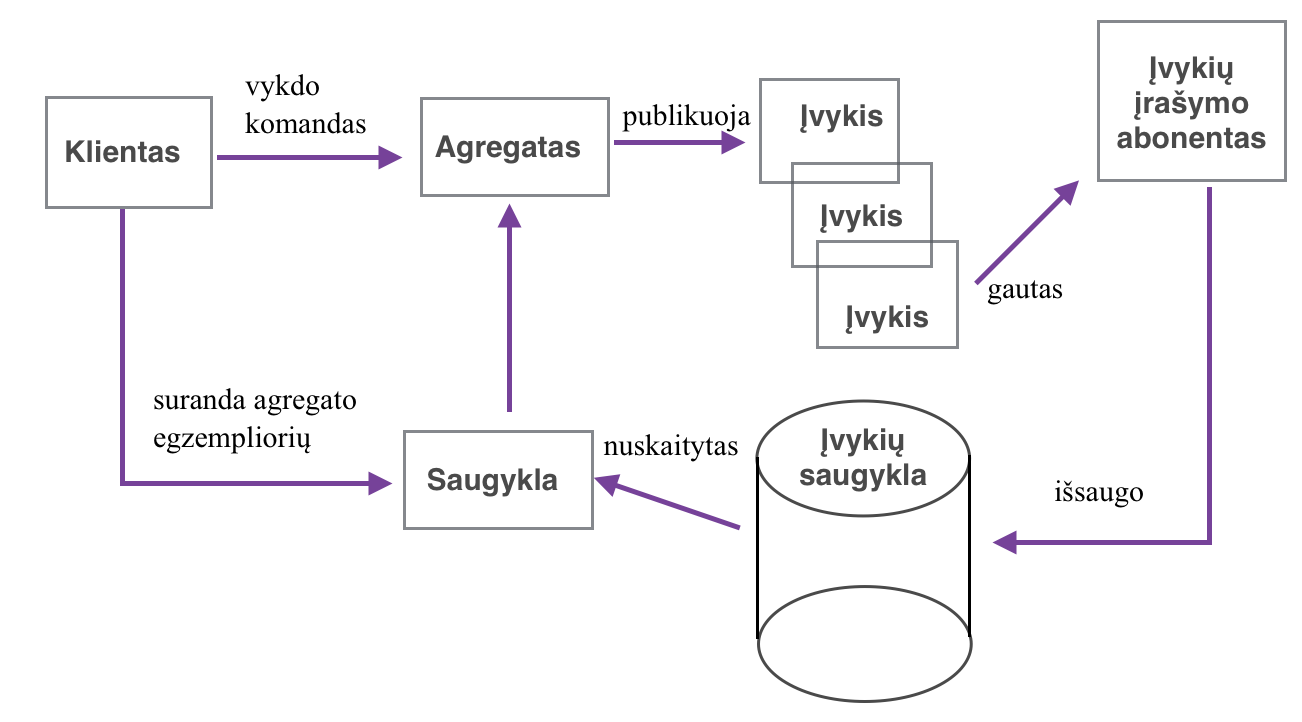
\includegraphics[width=0.9\linewidth]{pics/es.png}
	\caption{Įvykių kaupimo aukšo lygio reprezentacija}
	\label{pic:es}
\end{figure}

\subsubsection{Momentinė kopija}

Ilgame periode sistemoje susikaupia daugybė įvykių. Atkuriant agregato būseną reikia atkartoti šimtus, tūkstančius ar net milijonus įvykių. Tai tampa šio modelio silpnąja puse, nes įvykių atkartojimas užtrunka vis ilgiau sistemai plečiantis.

Tačiau šio duomenų kamsčio galima išvengti naudojant agregato būsenos momentines kopijas. Tam tikrame įvykių saugyklos istorijos taške yra padaroma agregato būsenos kopija. Serializuota agregato būsena yra įrašoma į įvykių saugyklą. Nuo to momento, agregatas yra atkuriamas pirmiausia naudojantis naujausia jo būsenos momentine kopija ir tik po to atkartojami visi naujesni įvykiai.

Momentinės kopijos nėra atkuriamos atsitiktinai. Jos gali būti kuriamos kas apibrėžtą skaičių įvykių. Šis skaičius turėtų būti parinktas analizuojant domeno sritį bei sistemą ir radus optimalų variantą. Tikėtinai gali būti 50 arba 100 įvykių tarp momentinių kopijų.

\subsubsection{Įvykių kaupimo privalumai ir trūkumai}

Kaip saugojimo mechanizmas, įvykių kaupimas stipriai skiriasi ir pakeičia ORM\footnote{http://www.orm.net/} įrankį. Kadangi įvykiai dažnai įrašomi kaip dvejetainės reprezentacijos, jie negali būti optimaliai naudojami užklausoms atlikti. Faktiškai įvykių kaupimu pagrįstoms saugykloms tereikia vienos operacijos - gauti įrašus pagal unikalią agregato tapatybę. To pasekoje užklausom daryti reikia kito kelio. Dažniausiai tam pasirenkamas CQRS\footnote{http://martinfowler.com/bliki/CQRS.html} principas. 

Įvykių kaupimas verčia kitaip mąstyti apie domeno modelį. Įvykių istorija gali padėti surasti bei ištaisyti sistemos defektus bei klaidas. Derinimas naudojant istoriją visų veiksmų, kurie nutiko sistemoje, turi didžiulį pranašumą. Įvykių kaupimas gali vesti prie didelio našumo domeno modelių, tai yra palaikyti ypač didelį skaičių operacijų per sekundę. Pavyzdžiui, įrašymas į vieną duomenų saugyklos lentelę yra ypač greitas. Negana to, tai leidžia CQRS užklausų modelį išplėsti horizontaliai, nes duomenų šaltinio atnaujinimai įvykdomi fone, kai įvykių saugykla yra atnaujinama naujais įvykiais.

\subsubsection{Įvykių srautas}

Pagal \cite{Bass:2007:Mythbusters}, įvykių srautas yra eilė pagal laiką surikiuotų įvykių, pavyzdžiui akcijų rinkos srautas.

Įvykių srautas kaip duomenų srauto tipas formaliai atrodo kaip pora (s, t), kur s yra seka surikiuotų sąrašo įvykių, o t yra seka laiko intervalų ir kiekvienas intervalas yra netuščias.

Tokio duomenų srauto pavyzdžiai gali būti:

\begin{itemize}

	\item akcijų kursas,

	\item paspaudimų srautas,

	\item tinklo srautas,

	\item GPS\footnote{http://en.wikipedia.org/wiki/Global\_Positioning\_System} duomenys.

\end{itemize}

Įvykių srauto apdorojimas pagal atsitikimo laiką turi privalumų:

\begin{itemize}

	\item įvykių apdorojimo algoritmai naudoja mažai atminties, nes jiems nereikia prisiminti daug įvykių;

	\item algoritmai gali būti labai greiti;

	\item gavus įvykį, skaičiavimai atliekami iškart, todėl galima perduoti rezultatą kitam skaičiavimui ir pamiršti įvykį.

\end{itemize}

Įvykių srauto apdorojimas labiau akcentuoja didelio našumo duomenų gavimą ir matematinių algoritmų pritaikymą įvykių duomenims. Taip pat įvykių srautai įprastai pritaikomi konkrečiai sistemai ar organizacijai.

\subsubsection{Įvykių kaupimas funkciniame programavime}

Vaughn Vernon pateikia keletą pastebėjimų apie įvykių kaupimą funkciniame programavime, kurie gali būti naudingi atliekant projektinius sprendimus bei eksperimentinį tyrimą:

\begin{itemize}

	\item Agregatas projektuojamas kaip nekintantis būsenos įrašas kartu su funkcijomis, kurios keičia būseną. Šios funkcijos paprasčiausiai priima būsenos įrašą ir įvykių argumentus ir gražina naują būsenos įrašą kaip rezultatą. Tokios funkcijos atrodo:

\begin{lstlisting}

	Func<Busena, Ivykis, Busena>

\end{lstlisting}

	\item Dabartinė agregato būsena gali būti apibrėžta kaip suskleidimas į kairę visų praeities įvykių, kurie yra perduodami būseną keičiančiai funkcijai.

	\item Agregato metodai gali būti išreikšti kaip kolekcija funkcijų be būsenos.

	\item Įvykių saugykla gali būti suvokiama bei naudojama kaip funkcinė duomenų bazė, nes ji perduoda argumentus funkcijoms, kurios keičia agregato būseną. Momentinės kopijos įvykių saugykloje primena įsiminimą atmintyje\footnote{http://en.wikipedia.org/wiki/Memoization} funkciniame programavime.

\end{itemize}

\subsection{Monados}

\subsubsection{Terminas}

Funkciniame programavime monada yra struktūra, kuri atspindi skaičiavimus, apibrėžtus kaip seka žingsnių. Tipas kartu su monados struktūra apibrėžia ką reiškia vykdyti operacijas viena po kitos bei naudoti to pačio tipo įdėtines funkcijas. Tai leidžia kurti komandų grandines, kurios pažingsniui apdoroja informaciją, kur kiekvienas veiksmas yra dekoruojamas naujomis apdorojimo taisyklėmis, kurias apibrėžia monada \cite{OSullivan:2008:RWH:1523280}.

taisykles?

\subsection{Išvados}

Literatūros analizės metu remiantis kitų autorių patirtimi:

\begin{itemize}

\item išnagrinėtas funkcinis-reaktyvus programavimas,

\item išnagrinėtas įvykių kaupimo principas,

\item išnagrinėti įvykių srautai,

\item susipažinta su įvykių kaupimu funkciniame programavime,

\item susipažinta su monadomis,

\item įvaldyta sąvokų sistema, susijusi su nagrinėjama tematika.

\end{itemize}
